%%%%%%%%%%%%%%%
% English application CV
% Compile with XeLaTeX
\documentclass[a4paper,10pt]{article}

\usepackage[a4paper,left=1.18cm,right=1.18cm,top=0.68cm,bottom=0.72cm]{geometry}
\usepackage{graphicx}
\usepackage{enumitem}
\usepackage{tabularx}
\usepackage{hyperref}
\usepackage{xcolor}
\usepackage{fontspec}
\usepackage{setspace}
\usepackage[fixed]{fontawesome5}

\setmainfont[
  Path=/System/Library/Fonts/Supplemental/,
  UprightFont={Times New Roman.ttf},
  BoldFont={Times New Roman Bold.ttf},
  ItalicFont={Times New Roman Italic.ttf},
  BoldItalicFont={Times New Roman Bold Italic.ttf}
]{Times New Roman.ttf}
\setsansfont[
  Path=/System/Library/Fonts/Supplemental/,
  UprightFont={Times New Roman.ttf},
  BoldFont={Times New Roman Bold.ttf},
  ItalicFont={Times New Roman Italic.ttf},
  BoldItalicFont={Times New Roman Bold Italic.ttf}
]{Times New Roman.ttf}
\setmonofont[
  Path=/System/Library/Fonts/Supplemental/,
  UprightFont={Times New Roman.ttf},
  BoldFont={Times New Roman Bold.ttf},
  ItalicFont={Times New Roman Italic.ttf},
  BoldItalicFont={Times New Roman Bold Italic.ttf},
  Scale=0.96
]{Times New Roman.ttf}

\definecolor{rulegray}{HTML}{D8D2C8}
\definecolor{markerred}{HTML}{8A1538}
\definecolor{deepred}{HTML}{8A1538}
\definecolor{softgray}{HTML}{E6E0D6}
\definecolor{textgray}{HTML}{333333}

\setstretch{1.0}
\setlength{\parindent}{0pt}
\setlength{\parskip}{1.2pt}
\setlist[itemize]{leftmargin=1.15em,itemsep=1.0pt,topsep=1.0pt,parsep=0pt}
\hypersetup{hidelinks,colorlinks=false}
\pagestyle{empty}

\newcommand{\cvicon}[1]{\textcolor{deepred}{#1}}

\newcommand{\sectionhead}[1]{%
  \par\addvspace{9pt}%
  \noindent{\fontsize{14.2}{15.4}\selectfont\bfseries #1\par}%
  \nobreak\vspace{2pt}%
  \nointerlineskip\hbox{\textcolor{deepred}{\rule{2.4em}{0.7pt}}\textcolor{rulegray}{\rule{\dimexpr\textwidth-2.4em\relax}{0.45pt}}}%
  \nobreak\vspace{3pt}\nointerlineskip
}
\newcommand{\contacticon}[1]{\textcolor{deepred}{#1}\hspace{0.34em}}
\newcommand{\role}[1]{\textbf{\textcolor{textgray}{#1}}}
\newcommand{\dateright}[1]{\hfill{\small\textcolor{textgray}{#1}}}
\newcommand{\paperitem}[4]{%
  \noindent\makebox[1.0em][l]{\textcolor{markerred}{\small\faBookmark}}%
  \begin{minipage}[t]{\dimexpr\textwidth-8.0em\relax}\raggedright\textbf{#1}\end{minipage}%
  \makebox[7.0em][r]{\small\textcolor{textgray}{#2}}\par\vspace{3pt}
  \hspace*{1.0em}\begin{minipage}[t]{\dimexpr\textwidth-1.0em\relax}
    #3\\[-1pt]
    {\normalsize #4}
  \end{minipage}\par\vspace{2.5pt}
}

\begin{document}

\noindent\begin{minipage}[t]{0.775\textwidth}
  {\fontsize{18.5}{20.5}\selectfont\bfseries Cheng Chen}\\[0.2pt]
  {\fontsize{10.8}{12.4}\selectfont\textcolor{deepred}{Communication Engineering Undergraduate}}\\[0.2pt]
  {\fontsize{12.0}{13.6}\selectfont\bfseries Tongji University}\\[3pt]
  {\fontsize{11.2}{12.8}\selectfont
  \begin{tabularx}{\linewidth}{@{}>{\raggedright\arraybackslash}X>{\raggedright\arraybackslash}X@{}}
    \contacticon{\faEnvelope}\href{mailto:2351445@tongji.edu.cn}{2351445@tongji.edu.cn} &
    \contacticon{\faEnvelope}\href{mailto:chenceason10@gmail.com}{chenceason10@gmail.com} \\
    \contacticon{\faGlobe}\href{https://ceasonen.github.io}{ceasonen.github.io} &
    \contacticon{\faGithub}\href{https://github.com/ceasonen}{github.com/ceasonen} \\
    \contacticon{\faUniversity}Major rank 2/85 &
    \contacticon{\faMapMarker}Shanghai, China
  \end{tabularx}}
\end{minipage}%
\hfill%
\begin{minipage}[t]{0.16\textwidth}
  \raggedleft
  \vspace{0.00cm}
  \setlength{\fboxsep}{0pt}\setlength{\fboxrule}{0.35pt}%
  \fcolorbox{softgray}{white}{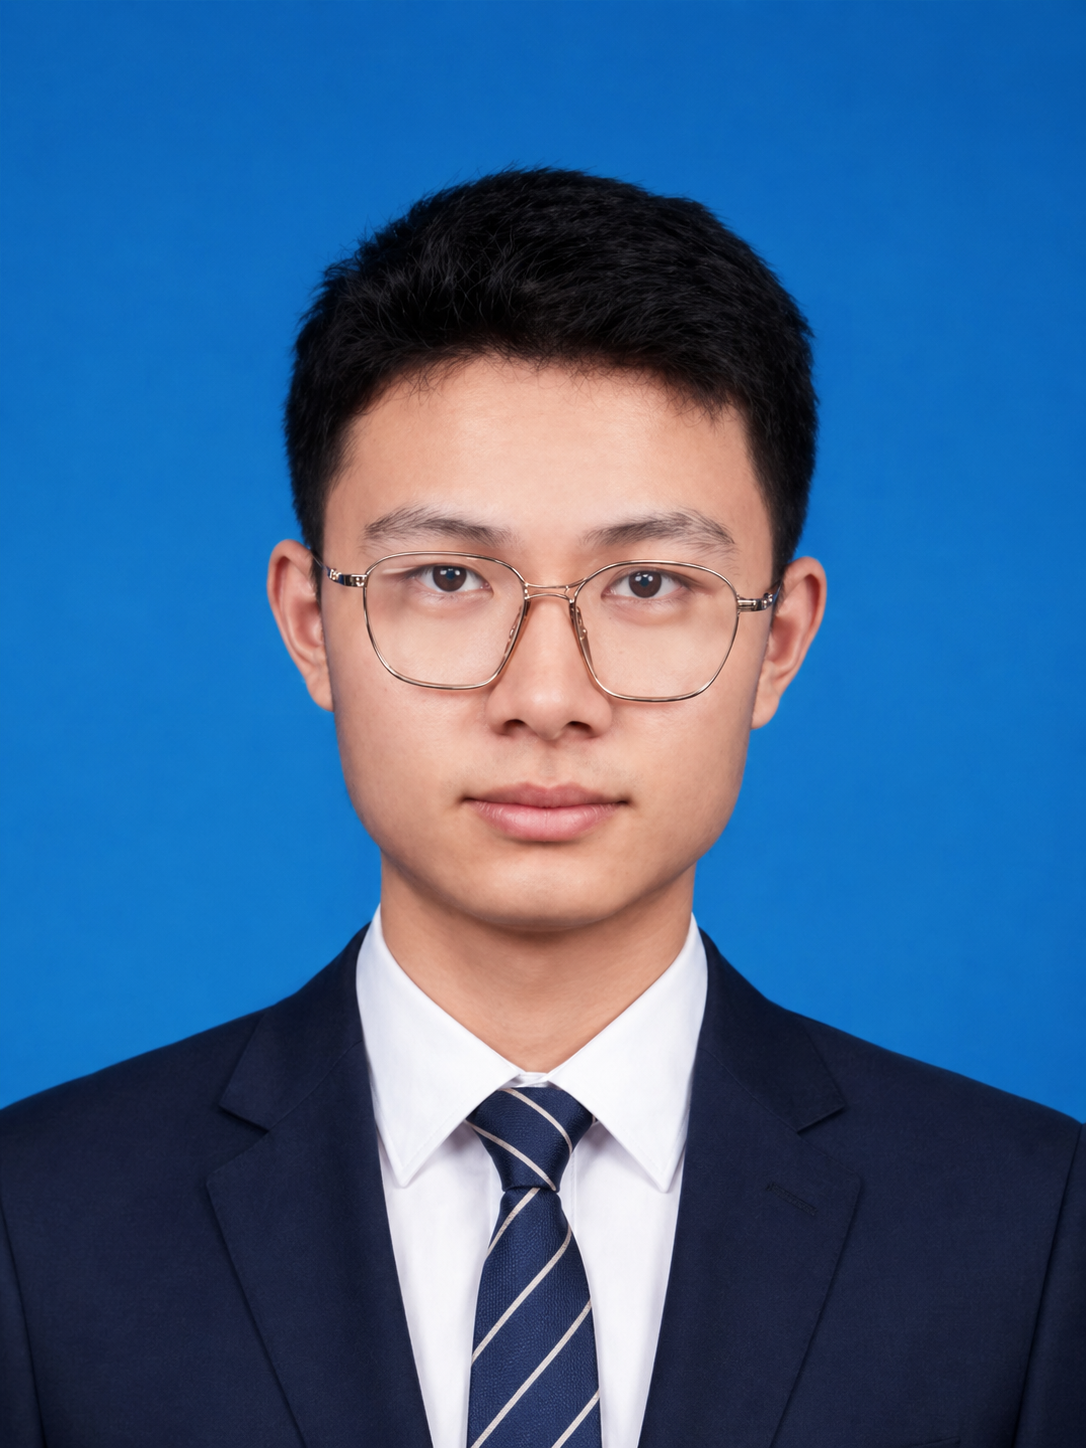
\includegraphics[width=2.25cm]{me.png}}
\end{minipage}\par\vspace{2pt}

\sectionhead{Summary}
\begin{itemize}
  \item Communication Engineering undergraduate at Tongji University. Interests: multimodal learning, language models, embodied AI, and efficient AI.
  \item Accepted papers at \textbf{ACM MM} and \textbf{IJCAI}.
\end{itemize}

\sectionhead{Education}
\textbf{B.Eng. in Communication Engineering, Tongji University}, Shanghai \dateright{2023.09 \textendash Jun. 2027}\\[-1pt]
Expected graduation: Jun. 2027. Major rank: \textbf{2/85}; CET-6: \textbf{519}.

\sectionhead{Internships}
\textit{Research Intern}\\
\begin{tabularx}{\textwidth}{@{}Xr@{}}
  \textbf{HKUST-GZ} & Sept. 2026 \textendash Present \\
  \textbf{Zhejiang University} & Jun. 2026 \textendash Sept. 2026 \\
  \textbf{Tongji University} & Oct. 2025 \textendash Jun. 2026 \\
\end{tabularx}

\sectionhead{Research}
\paperitem{If You Hear It, Help Find It: Orthogonal Knowledge Distillation for Open-Vocabulary Audio-Visual Event Localization}{ACM MM 2026}
{\role{Published; co-first author (listed second).}\quad\href{https://doi.org/10.1145/3767308.3835302}{[DOI]}}
{Proposed reliability-aware asymmetric distillation for open-vocabulary audio-visual event localization. The method isolates weak-audio features in an orthogonal auxiliary subspace and improves F1@0.5 by 2.7 points overall and 3.4 points on unseen categories.}

\paperitem{OrthKD: Extracting Generalized Clinical Knowledge from Heterogeneous Teachers for Lightweight Deployment}{IJCAI 2026}
{\role{Accepted; co-first author.}}
{Developed heterogeneous multi-teacher distillation for diabetic-retinopathy screening. A 5.4M-parameter student reached 0.885 QWK on EyePACS and improved zero-shot Messidor-2 QWK from 0.507 to 0.728.}

\sectionhead{Awards}
\begin{tabularx}{\textwidth}{@{}>{\raggedright\arraybackslash}Xr@{}}
  National First Prize, China Robot and Artificial Intelligence Competition, Team Leader & 2026 \\
  National Second Prize, Global Campus Artificial Intelligence Algorithm Elite Competition, Team Leader & 2025 \\
  National Third Prize, National Undergraduate Embedded Chip and System Design Contest, Team Leader & 2025 \\
  Tongji University BULL Scholarship, First-Class equivalent & 2026 \\
  Tongji University Outstanding Student Scholarship & 2023--2024, 2024--2025 \\
\end{tabularx}

\sectionhead{Academic Service}
\textbf{Reviewer:} ICLR, PRCV, ICME, IJCNN, AAAI.

\sectionhead{Skills}
\begin{itemize}
  \item \role{Programming:} \textbf{Python}, \textbf{C/C++}, \textbf{Verilog}. \role{Framework:} \textbf{PyTorch}.
  \item \role{Tools:} \textbf{Git}, \textbf{Linux}, \textbf{LaTeX}, \textbf{OpenAI Codex}, and \textbf{Claude Code}.
  \item \role{Writing:} English research-paper reading; academic and project writing.
  \item \role{Research motivation:} I enjoy learning new topics and developing them into concrete research results.
  \item \role{Outside lab:} \cvicon{\faFutbol} Football (Barça \& Arsenal), cycling, music.
\end{itemize}

\end{document}
